%-------------------------------------------------------------------------------
%-------------------------------------------------------------------------------
%-------------------------------------------------------------------------------
\chapter{Algorithme de Tarjan}
%-------------------------------------------------------------------------------
%-------------------------------------------------------------------------------
\thispagestyle{empty}
%-------------------------------------------------------------------------------
%-------------------------------------------------------------------------------
%-------------------------------------------------------------------------------
{\it On cherche à déterminer les composantes fortement connexes d'un graphe {\bf non orienté} : ce sont les classes d'équivalence pour la relation définie par $s\sim t$ si et seulement si il existe un chemin de $s$ vers $t$ et un chemin de $t$ vers $s$.

On pourra illustrer les fonctions écrites pour les deux graphes suivants :
%-------------------------------------------------------------------------------
\begin{figure}[!htb]
\centering
\begin{subfigure}[b]{0.40\textwidth}
\centering
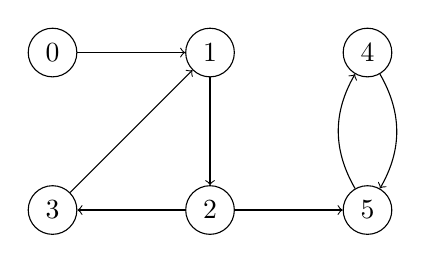
\begin{tikzpicture}[every node/.style={draw,circle}]
\node (s0) at (0,0) {0};
\node (s1) at (2,0) {1};
\node (s2) at (2,-2) {2};
\node (s3) at (0,-2) {3};
\node (s4) at (4,0) {4};
\node (s5) at (4,-2) {5};
\draw[->] (s0) -- (s1);
\draw[->] (s1) -- (s2);
\draw[->] (s2) -- (s3);
\draw[->] (s3) -- (s1);
\draw[->] (s2) -- (s5);
\draw[->] (s5) edge[bend left] (s4);
\draw[->] (s4) edge[bend left] (s5);
\end{tikzpicture}
\caption{\label{fig:g1}}
\end{subfigure}
\quad
\begin{subfigure}[b]{0.40\textwidth}
\centering
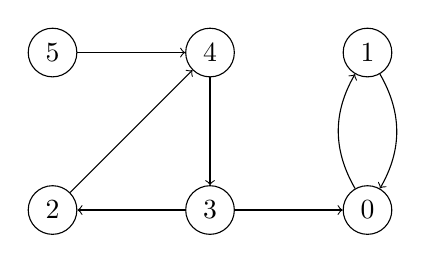
\begin{tikzpicture}[every node/.style={draw,circle}]
\node (s0) at (0,0) {5};
\node (s1) at (2,0) {4};
\node (s2) at (2,-2) {3};
\node (s3) at (0,-2) {2};
\node (s4) at (4,0) {1};
\node (s5) at (4,-2) {0};
\draw[->] (s0) -- (s1);
\draw[->] (s1) -- (s2);
\draw[->] (s2) -- (s3);
\draw[->] (s3) -- (s1);
\draw[->] (s2) -- (s5);
\draw[->] (s5) edge[bend left] (s4);
\draw[->] (s4) edge[bend left] (s5);
\end{tikzpicture}
\caption{\label{fig:g2}}
\end{subfigure}
\caption{\protect\subref{fig:g1} Graphe $G_1$, \protect\subref{fig:g2} Graphe $G_2$}
\end{figure}
%-------------------------------------------------------------------------------
%-------------------------------------------------------------------------------
Ils correspondent au même graphe avec des numérotations des sommets différentes.

\medskip

La représentation des graphes devra donner les fonctions

\begin{lstlisting}
taille : graphe -> int 
voisins : graphe -> int -> int list 
\end{lstlisting}

Dans les exemples on supposera que les voisins sont donnés par ordre croissant.

\medskip

Pour les calculs de complexité, on supposera que les graphes sont définis par des tableaux d'adjacence, le type \type{graphe} sera alors \type{int list array}. 
Le graphe $G_1$ sera alors représenté par 
%-------------------------------------------------------------------------------
\begin{lstlisting}
let g1 = [|[1]; [2]; [3; 5]; [1]; [5]; [4]|];;
\end{lstlisting}
%-------------------------------------------------------------------------------
}
%-------------------------------------------------------------------------------
%-------------------------------------------------------------------------------
%-------------------------------------------------------------------------------
\section{Algorithme de Tarjan} 
%-------------------------------------------------------------------------------
%-------------------------------------------------------------------------------
%-------------------------------------------------------------------------------
Nous allons écrire l'algorithme de Tarjan par étapes.

%-------------------------------------------------------------------------------
%-------------------------------------------------------------------------------
\subsection{Composantes connexes d'un graphe non orienté} 
%-------------------------------------------------------------------------------
%-------------------------------------------------------------------------------
On part du parcours en profondeur classique (sans utiliser \type{List.iter}) pour déterminer les composantes connexes d'un graphe non orienté..
%-------------------------------------------------------------------------------
\begin{lstlisting}
let composantes g = 
  let n = taille g in
  let cc = Array.make n (-1) in
  let num = ref 0 in
  let rec voir s =
    let rec aux liste = 
      match liste with
      |[] -> ()
      |t::q -> if cc.(t) = -1 then voir t;
               aux q in
    cc.(s) <- !num;
    aux (voisins g s) in
  for i = 0 to (n-1) do 
    if pref.(i) = -1 
    then begin voir i;
               num := !num + 1 end done;
  cc;;
\end{lstlisting}
%-------------------------------------------------------------------------------
\begin{figure}[ht]
\begin{center}
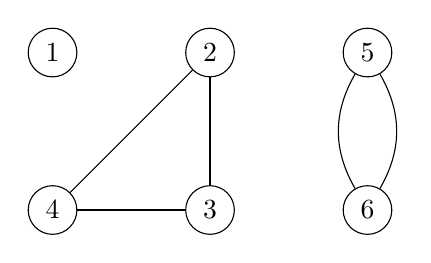
\begin{tikzpicture}[every node/.style={draw,circle}]
\node (s0) at (0,0) {1};
\node (s1) at (2,0) {2};
\node (s2) at (2,-2) {3};
\node (s3) at (0,-2) {4};
\node (s4) at (4,0) {5};
\node (s5) at (4,-2) {6};
\draw (s1) -- (s2);
\draw (s2) -- (s3);
\draw (s3) -- (s1);
\draw (s5) edge[bend left] (s4);
\draw (s4) edge[bend left] (s5);
\end{tikzpicture}
\caption{Graphe non orienté $G_0$}
\end{center}
\end{figure}
%-------------------------------------------------------------------------------
Le tableau des numéros des composantes sert de contrôle des éléments vus.

Pour le graphe $G_0$, la fonction renvoie \type{[|0; 1; 1; 1; 2; 2|]}
%-------------------------------------------------------------------------------
%-------------------------------------------------------------------------------
\subsection{Ordre préfixe} 
%-------------------------------------------------------------------------------
%-------------------------------------------------------------------------------
On commence part modifier le parcours en profondeur pour numéroter les sommets dans l'ordre où on commence à les explorer, c'est l'ordre infixe.
%-------------------------------------------------------------------------------
%-------------------------------------------------------------------------------
\begin{Exercise}\it 
Écrire une fonction \type{prefixe : graphe -> int array} qui calcule cette numérotation.
\end{Exercise} 
%--------------------------------------------------------------------------
\begin{Answer}
Le principal changement avec le calcul des composantes connexes est le moment où on incrémente le numéro.
\begin{lstlisting}
let prefixe g = 
  let n = taille g in
  let pref = Array.make n (-1) in
  let num = ref 0 in
  let rec voir s =
    let rec aux liste = 
      match liste with
      |[] -> ()
      |t::q -> if pref.(t) = -1 then voir t;
               aux q in
    pref.(s) <- !num;
    num := !num +1;
    aux (voisins g s) in
  for i = 0 to (n-1) 
    do if pref.(i) = -1 then voir i done;
  pref;;
\end{lstlisting}
\end{Answer} 
%-------------------------------------------------------------------------------
\begin{lstlisting}
# prefixe g1
- : int array = [|0; 1; 2; 3; 5; 4|]
# prefixe g2
- : int array = [|0; 1; 2; 4; 3; 5|]
\end{lstlisting}
%-------------------------------------------------------------------------------
%-------------------------------------------------------------------------------
\subsection{Minimum de retour} 
%-------------------------------------------------------------------------------
%-------------------------------------------------------------------------------
On peut remarquer que, parmi les sommets d'une même composante fortement connexe (CFC), il en existe un particulier, c'est celui qui est visité en premier (son numéro est minimum), c'est la racine de la composante. Bien entendu la racine d'une composante dépend de l'ordre de parcours des sommets. 

Lors de l'exploration depuis la racine, tous les sommet de la CFC vont être visités et le parcours va, de plus, explorer des sommets de la CFC déjà vus car il existe un chemin vers la racine. 

On va changer le numéro en numéro minimum, associé à chaque sommet : 
%-------------------------------------------------------------------------------
\begin{itemize}
    \item quand un sommet est visité, on attribue initialement la valeur d'ordre de visite au minimum
    \item quand on explore ses voisins, les voisins non encore vus sont visités ce qui calcule une valeur pour le minimum, les voisins déjà vus ont déjà un minimum
    \item à chaque voisin de $s$ on met à jour le minimum de $s$ en le remplaçant par celui du voisin s'il est inférieur.
\end{itemize}
%-------------------------------------------------------------------------------
Par exemple l'exploration de $G_1$ donne
%-------------------------------------------------------------------------------
\def\f{$\rightarrow$}
\begin{center}
\begin{tabular}{ccccccccccc|l}
&&&&&&&&&&&\type{mini} \\
\hline
0&  & &  & &  & &  & &  & &\type{[| 0; -1; -1; -1; -1; -1|]}\\
0&\f&1&  & &  & &  & &  & &\type{[| 0;  1; -1; -1; -1; -1|]}\\
0&\f&1&\f&2&  & &  & &  & &\type{[| 0;  1;  2; -1; -1; -1|]}\\
0&\f&1&\f&2&\f&3&  & &  & &\type{[| 0;  1;  2;  3; -1; -1|]}\\
0&\f&1&\f&2&\f&3&\f&1&  & &\type{[| 0;  1;  2;  3; -1; -1|]}\\
0&\f&1&\f&2&\f&3&  & &  & &\type{[| 0;  1;  2;  1; -1; -1|]}\\
0&\f&1&\f&2&  & &  & &  & &\type{[| 0;  1;  1;  1; -1; -1|]}\\
0&\f&1&\f&2&\f&5&  & &  & &\type{[| 0;  1;  1;  1;  4; -1|]}\\
0&\f&1&\f&2&\f&5&\f&4&  & &\type{[| 0;  1;  1;  1;  4;  5|]}\\
0&\f&1&\f&2&\f&5&\f&4&\f&5&\type{[| 0;  1;  1;  1;  4; 5|]}\\
0&\f&1&\f&2&\f&5&\f&4&  & &\type{[| 0;  1;  1;  1;  4; 4|]}\\
0&\f&1&\f&2&\f&5&  & &  & &\type{[| 0;  1;  1;  1;  4; 4|]}\\
0&\f&1&\f&2&  & &  & &  & &\type{[| 0;  1;  1;  1;  4; 4|]}\\
0&\f&1&  & &  & &  & &  & &\type{[| 0;  1;  1;  1;  4; 4|]}\\
0&  & &  & &  & &  & &  & &\type{[| 0;  1;  1;  1;  4; 4|]}\\
\end{tabular}
\end{center}
%-------------------------------------------------------------------------------
%-------------------------------------------------------------------------------
\begin{Exercise}\it 
Écrire une fonction \type{minimum : graphe -> int array} qui calcule cette numérotation.
\end{Exercise} 
%--------------------------------------------------------------------------
\begin{Answer}
Une ligne à ajouter
\begin{lstlisting}
let minimum g = 
  let n = taille g in
  let mini = Array.make n (-1) in
  let num = ref 0 in
  let rec voir s =
    let rec aux liste = 
      match liste with
      |[] -> ()
      |t::q -> if mini.(t) = -1 then voir t;
               if mini.(t) < mini.(s) then mini.(s) <- mini.(t);
               aux q in
    mini.(s) <- !num;
    num := !num +1;
    aux (voisins g s) in
  for i = 0 to (n-1) 
    do if mini.(i) = -1 then voir i done;
  mini;;
\end{lstlisting}
\newpage
\end{Answer} 
%-------------------------------------------------------------------------------
\begin{lstlisting}
# minimum g1
- : int array = [|0; 1; 1; 1; 4; 4|]
\end{lstlisting}
%-------------------------------------------------------------------------------
%-------------------------------------------------------------------------------
\subsection{Restriction des cas} 
%-------------------------------------------------------------------------------
%-------------------------------------------------------------------------------
Malheureusement la fonction ci-dessus ne donne pas les composantes fortement connexes dans tous les cas.
%-------------------------------------------------------------------------------
\begin{lstlisting}
# minimum g2
- : int array = [|0; 0; 0; 0; 0; 0|]
\end{lstlisting}
%-------------------------------------------------------------------------------
Voici le détail du parcours
%-------------------------------------------------------------------------------
\def\f{$\rightarrow$}
\begin{center}
\begin{tabular}{ccccccccccc|l}
&&&&&&&&&&&\type{mini} \\
\hline
0&  & &  & &  & &  & &  & &\type{[| 0; -1; -1; -1; -1; -1|]}\\
0&\f&1&  & &  & &  & &  & &\type{[| 0;  1; -1; -1; -1; -1|]}\\
0&\f&1&\f&0&  & &  & &  & &\type{[| 0;  1; -1; -1; -1; -1|]}\\
0&\f&1&  & &  & &  & &  & &\type{[| 0;  0; -1; -1; -1; -11|]}\\
0&  & &  & &  & &  & &  & &\type{[| 0;  0; -1; -1; -1; -1|]}\\
2&  & &  & &  & &  & &  & &\type{[| 0;  0;  2; -1; -1; -1|]}\\
2&\f&4&  & &  & &  & &  & &\type{[| 0;  0;  2; -1;  3; -1|]}\\
2&\f&4&\f&3&  & &  & &  & &\type{[| 0;  0;  2;  4;  3; -1|]}\\
2&\f&4&\f&3&\f&0&  & &  & &\type{[| 0;  0;  2;  4;  3; -1|]}\\
2&\f&4&\f&3&  & &  & &  & &\type{[| 0;  0;  2;  0;  3; -1|]}\\
2&\f&4&\f&3&\f&2&  & &  & &\type{[| 0;  0;  2;  0;  3; -1|]}\\
2&\f&4&\f&3&  & &  & &  & &\type{[| 0;  0;  2;  0;  3; -1|]}\\
2&\f&4&  & &  & &  & &  & &\type{[| 0;  0;  2;  0;  0; -1|]}\\
2&  & &  & &  & &  & &  & &\type{[| 0;  0;  0;  0;  0; -1|]}\\
5&  & &  & &  & &  & &  & &\type{[| 0;  0;  0;  0;  0;  5|]}\\
5&\f&4&  & &  & &  & &  & &\type{[| 0;  0;  0;  0;  0;  5|]}\\
5&  & &  & &  & &  & &  & &\type{[| 0;  0;  0;  0;  0;  0|]}\\
\end{tabular}
\end{center}
%-------------------------------------------------------------------------------

Le problème ici est que, lors de l'exploration de 3, le sommet à un voisin 0 qui a déjà été complètement exploré et qui ne peut donc pas accéder à 3 ; de même pour 5 qui admet 4 comme voisin.

Pour éviter le problème on peut ajouter un tableau de booléen qui permet de marquer comme finis les sommets dont l'exploration est achevée ; on ne mettra à jour le minimum avec un voisin que lorsque le voisin n'est pas fini. 

Cette dernière règle est trop rigide, lorsque l'on parcourt un sommet $t$ depuis $s$ avec \type{mini.(t) = -1}, le sommet $t$ aura été complètement visité au moment de la mise à jour de \type{mini.(s)}, alors que, dans ce cas, il est nécessaire de mettre à jour.
%-------------------------------------------------------------------------------
%-------------------------------------------------------------------------------
\begin{Exercise}\it 
Écrire une fonction \type{minimum1 : graphe -> int array} qui calcule la numérotation avec le test d'achèvement du parcours en modifiant la règle rigide.
\end{Exercise} 
%--------------------------------------------------------------------------
\begin{Answer}

Une nouvelle variable, un test supplémentaire et une nouvelle affectation.

On ne fait le test de \type{fini.(t)} que pour les sommets dont l'exploration à déjà commencé.
\begin{lstlisting}
let minimum1 g = 
  let n = taille g in
  let mini = Array.make n (-1) in
  let fini = Array.make n false in
  let num = ref 0 in
  let rec voir s =
    let rec aux liste = 
      match liste with
      |[] -> ()
      |t::q -> if mini.(t) = -1 
               then begin voir t;
                    if mini.(t) < mini.(s) 
                    then mini.(s) <- mini.(t) end
                else if not fini.(t) && mini.(t) < mini.(s) 
                     then mini.(s) <- mini.(t);
               aux q in
    mini.(s) <- !num;
    num := !num +1;
    aux (voisins g s);
    fini.(s) <- true in
  for i = 0 to (n-1) 
    do if mini.(i) = -1 then voir i done;
  mini;;
\end{lstlisting}
\end{Answer} 
%-------------------------------------------------------------------------------
\begin{lstlisting}
# minimum1 g1
- : int array = [|0; 1; 1; 1; 4; 4|]
# minimum1 g2
- : int array = [|0; 0; 2; 2; 2; 5|]
\end{lstlisting}
%-------------------------------------------------------------------------------
%-------------------------------------------------------------------------------
\subsection{Une pile} 
%-------------------------------------------------------------------------------
%-------------------------------------------------------------------------------
Encore une fois, les efforts faits ne suffisent pas. On le constate sur le graphe $G_3$ : il y a plusieurs indices mais une seule CFC.

%-------------------------------------------------------------------------------
\begin{figure}[ht]
\begin{center}
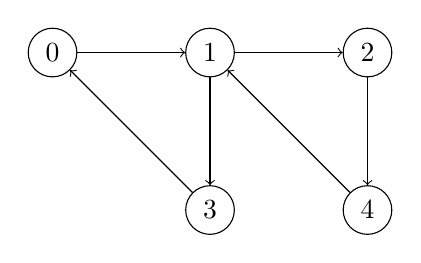
\begin{tikzpicture}[every node/.style={draw,circle}]
\node (s0) at (0,0) {0};
\node (s1) at (2,0) {1};
\node (s2) at (4,0) {2};
\node (s3) at (2,-2) {3};
\node (s4) at (4,-2) {4};
\draw[->] (s0) -- (s1);
\draw[->] (s1) -- (s2);
\draw[->] (s1) -- (s3);
\draw[->] (s2) -- (s4);
\draw[->] (s3) -- (s0);
\draw[->] (s4) -- (s1);
\end{tikzpicture}
\caption{Graphe $G_0$}
\end{center}
\end{figure}
%-------------------------------------------------------------------------------
Le problème ici est que, lors de l'exploration de 1, le parcours visite 2 qui revient à 1 alors que 1 n'a pas encore vu son minimum diminuer : il le sera en visitant 3 puis 0.

L'idée suivante est de calculer directement les CFC en utiliser les valeurs du minimum pour reconnaître les racines. En effet celles-ci ne peuvent pas voir leur valeur du minimum diminuer, elles sont caractérisées par l'égalité entre le minimum et la valeur de l'ordre préfixe (il faudra donc la conserver). Les sommets de la CFC associée sont alors qui succèdent à la racine {\bf mais qui ne sont pas encore dans une autre CFC}.

Pour obtenir ces points on va empiler les sommets visités et, lorsque l'on a un sommet \type{s} pour lequel \type{pref(s) = mini.(s)} on dépile les sommets de la pile jusqu'à \type{s} : cela forme la CFC.
%-------------------------------------------------------------------------------
%-------------------------------------------------------------------------------
\begin{Exercise}\it 
Écrire une fonction \type{tarjan : graphe -> int list list} qui calcule la liste des composantes fortement connexes (codées sous forme de listes).
\end{Exercise} 
%--------------------------------------------------------------------------
\begin{Answer}
Beaucoup de variables \dots

On utilise une liste référencée comme pile.

On commence par une fonction qui découpe une pile selon un sommet lui appartenant.
\begin{lstlisting}
let jusqua x pile en_cours =
  let rec aux fait reste =
    match reste with
    |[] -> [], fait
    |t::q when t = x -> en_cours.(t) <- false; t::fait,q
    |t::q -> en_cours.(t) <- false; aux (t::fait) q
  in  aux [] pile;;
\end{lstlisting}

On peut alors écrire la fonction
\newpage
\begin{lstlisting}
let tarjan g = 
  let n = taille g in
  let pref = Array.make n (-1) in
  let mini = Array.make n (-1) in
  let en_cours = Array.make n false in
  let num = ref 0 in
  let cfc = ref [] in
  let pile = ref [] in 
  let rec voir s =
    let rec aux liste = 
      match liste with
      |[] -> ()
      |t::q -> if pref.(t) = -1 then voir t;
               if en_cours.(t) && mini.(t) < mini.(s) 
               then mini.(s) <- mini.(t);
               aux q 
    in pref.(s) <- !num;
    mini.(s) <- !num;
    num := !num +1;
    pile := s :: !pile;
    en_cours.(s) <- true;
    aux (voisins g s);
    if pref.(s) = mini.(s) 
    then begin let debut, fin = jusqua s !pile en_cours in 
         cfc := debut :: !cfc; 
         pile := fin end
  in for i = 0 to (n-1) 
    do if pref.(i) = -1 then voir i done;
  !cfc;;
\end{lstlisting}
\end{Answer} 
%-------------------------------------------------------------------------------
%-------------------------------------------------------------------------------
\begin{itemize}
    \item La preuve de l'algorithme est subtile (lire : je ne sais pas la faire).
    \item Par contre la complexité est assez simple : on fait un parcours en profondeur et on empile et dépile (une seule fois) les sommet on obtient une complexité en ${\cal O}\bigl(|S| + |A|\bigr)$, linéaire.
\end{itemize}

\newpage

%-------------------------------------------------------------------------------
%-------------------------------------------------------------------------------
%-------------------------------------------------------------------------------
\section{Quelques graphes} 
%-------------------------------------------------------------------------------
%-------------------------------------------------------------------------------
%-------------------------------------------------------------------------------
\subsection{Les catégories de Roget} 
%-------------------------------------------------------------------------------
%-------------------------------------------------------------------------------
Peter Mark Roget a publié, en 1851, un livre, le {\it Thesaurus of English Words ans Phrases}, qui renversait le principe d'un dictionnaire. Au lieu d'associer des catégories aux mots, le thesaurus associe des mots aux catégories. Le livre contient ainsi 1022 catégories (dans la seconde édition) qui contiennent des listes de mots les concernant.

Ce qui nous intéresse c'est que les catégories peuvent renvoyer à d'autres, sans que cela soit forcement réversible : on obtient ainsi un graphe orienté.

Ces données ont été traduites dans deux fichiers :
\begin{itemize}
    \item le fichiers \type{roget\_gr.ml} définit le graphe associé, \type{g}, sous la forme d'un tableau d'adjacence
    \item le fichiers \type{roget\_noms.ml} définit le tableau des noms des concepts, \type{noms}, \type{noms.(k)} contient le nom du concept correspondant au sommet $k$ du graphe.
\end{itemize}

On intègre les définitions par les instructions

\begin{lstlisting}
#use "chemin/vers/les/fichiers/roget_gr.ml";;
#use "chemin/vers/les/fichiers/roget_noms.ml";;
\end{lstlisting}

On pourra donc calculer les composantes fortement connexes
\begin{lstlisting}
let cfc_roget = tarjan g;;
\end{lstlisting}
%-------------------------------------------------------------------------------
%-------------------------------------------------------------------------------
\begin{Exercise}\it 
Déterminer la taille de la plus grande CFC.
\end{Exercise} 
%--------------------------------------------------------------------------
\begin{Answer}
\begin{lstlisting}
let rec max_lg liste k =
match liste with
|[] -> k
|t::q -> max_lg q (max k (List.length t));;

max_lg cfc_roget 0;;

904
\end{lstlisting}
\end{Answer} 
%-------------------------------------------------------------------------------
%-------------------------------------------------------------------------------
\begin{Exercise}\it 
Déterminer les catégories des composantes à trois éléments.
\end{Exercise} 
%--------------------------------------------------------------------------
\begin{Answer}
\begin{lstlisting}
let imprimer3 liste = 
if List.length liste = 3
then begin List.iter (fun k -> print_string (noms.(k)^" ")) liste; 
print_newline() end;;


List.iter imprimer3 cfc_roget;;
\end{lstlisting}
\newpage

\begin{lstlisting}
adolescence man woman 
plurality fraction zero 
idolatry pseudo-revelation revelation 
interpreter oracle sorcerer 
consanguinity paternity posterity 
\end{lstlisting}
\end{Answer} 
%-------------------------------------------------------------------------------
%-------------------------------------------------------------------------------
\subsection{Divisibilité et permutations} 
%-------------------------------------------------------------------------------
%-------------------------------------------------------------------------------
On considère l'ensemble $S$ des entiers de 0 à 999.

Les arêtes du graphes sont les couples $(p, q)$ tels que 
\begin{itemize}
    \item $p$ et $q$ sont des anagrammes $173 \rightarrow 317$, $7 \rightarrow 700$
    \item ou $p$ divise $q$, $153 \rightarrow 612$.
\end{itemize}
%-------------------------------------------------------------------------------
%-------------------------------------------------------------------------------
\begin{Exercise}\it 
Déterminer le graphe.
\end{Exercise} 
%--------------------------------------------------------------------------
\begin{Answer}
\begin{lstlisting}
\end{lstlisting}
\end{Answer} 
%-------------------------------------------------------------------------------
%-------------------------------------------------------------------------------
\begin{Exercise}\it 
Déterminer la CFC de taille maximale.
\end{Exercise} 
%--------------------------------------------------------------------------
\begin{Answer}
\begin{lstlisting}
\end{lstlisting}
\end{Answer} 
%-------------------------------------------------------------------------------
%-------------------------------------------------------------------------------






